\documentclass[tcc, capa]{texucpel}

\usepackage[utf8]{inputenc}
\usepackage[T1]{fontenc}
\usepackage{verbatim}
\usepackage{amsmath}
\usepackage{graphicx} % para inserir figuras

\usepackage{microtype} % detalhes de justificação e espaçamento
\usepackage{nowidow} % evita que a última linha de um parágrafo mude de pag.
\usepackage{paralist} % lista sem o espaçamento de uma linha entre itens
\usepackage{booktabs} % 'rules' em tabelas
\usepackage{multirow} % Mágicas com tabelas
\usepackage{amssymb} % checkmark
\usepackage{icomma} % corrigir decimais (exceto unidades SI)
\usepackage{fourier} % muda a fonte de matemática pra colidir menos com arial
\usepackage{nameref}
\usepackage{verbatim}
 \usepackage{float}
\usepackage{siunitx}
\usepackage{placeins}

\sisetup{
	detect-family = true,
	detect-shape = true,
	detect-weight = true,
	detect-mode = true,
	output-decimal-marker = {,},
	binary-units = true
}%



\newcommand{\esp}{ESP8266}
\newcommand{\esppci}{ESP-01}
\newcommand{\exehda}{EXEHDA}
\newcommand{\middleware}{\emph{middleware}}
\newcommand{\pic}{PIC}
\newcommand{\picm}{PIC18F4550}
\newcommand{\picf}{PIC18F}
\newcommand{\hc}{HC-05}
\newcommand{\meter}{\mbox{ubiMeter}}

\newcommand{\gambi}{\fontfamily{phv}\fontshape{n}\selectfont}
\newcommand{\media}{\(\textrm{\gambi{} Média (\si{\volt})}\)}
\newcommand{\desvio}{\(\textrm{\gambi{} Desvio Padrão}\)}
\newcommand{\maximo}{\(\textrm{\gambi{} Máximo (\si{\volt})}\)}
\newcommand{\minimo}{\(\textrm{\gambi{} Mínimo (\si{\volt})}\)}
\newcommand{\erromed}{\(\textrm{\gambi{} Erro médio}\)}
\newcommand{\erromax}{\(\textrm{\gambi{} Erro máximo}\)}

\unidade{Centro de Ciências Sociais e Tecnológicas}
\curso{Engenharia de Computação}
\nomecurso{Engenharia de Computação}
\titulocurso{Engenheiro de Computação.}

\title{Otimizando função de pontuação de docking molecular com uso de Support Vector Machine }

\author{de Campos}{Gianluca}
\vspace{1.2cm}

\advisor [Prof. Me.]{Mertins}{Luciano Edson}

\keyword{Otimização}
\keyword{Avaliação}
\keyword{Predição}

\begin{document}
\maketitle 
\renewcommand{\advisorname}
{Orientador}          
\sloppy
\fichacatalografica
\folhadeaprovacao
%Opcional
%\begin{dedicatoria}
%\end{dedicatoria}

%Opcional
\begin{agradecimentos}
\textbf{Agradecimentos} \\
Em primeiro lugar gostaria de agradecer ao apoio de meus familiares por ser possível estar aqui estudando nesta instituição, dando o máximo de suporte possível para que eu pudesse estar aqui hoje.

Agradeço também aos colegas de turma, em especial ao Marcos e Rociele, por me dar apoio na hora que mais precisei.

Também agradeço à colegas de trabalho, em especial Rodrigo Lima (vulgo Carioca) pela constante cobrança quanto aos prazos deste trabalho.

Em especial um agradecimento também ao meu professor orientador Luciano Edson Mertins, por se disponibilizar para me ajudar ao longo deste curso, auxiliando nas difíceis tarefas, estudo e também pelo monitoramento delas, para que pudesse desta forma, concluir o trabalho. Agradecer ao mesmo também, principalmente pela formação, tanto de aluno como futuro profissional.
\vspace{\baselineskip}
\end{agradecimentos}

%Opcional

\begin{epigrafe}{John Lennon}
"When I was 5 years old, my mother always told me that happiness was the key to life. When I went to school, they asked me what I wanted to be when I grew up. I wrote down ‘happy’. They told me I didn’t understand the assignment, and I told them they didn’t understand life."\\
\end{epigrafe}

\begin{abstract}
O processo de desenvolvimentode drogas mediceinais é demorado, custoso e em grande parte manual.
Para melhorar e condicionar uma droga a um efeito desejado, usa-se uma técnica chamada Docking Molecular, que consiste em realizar o atracamento entre uma estrutura denominada ligante e outra receptora, onde o resultado do atracamento, demonstra o grau de afinidade da ligação entre as mesmas.
Esta técnica está presente em diversos softwares, que exibem design da estrutura das moléculas, onde é possível efetuar a manipulação e aplicar ajustes para então estimar resultados.
Para este trabalho, é proposto como solução aplicar, com auxílio de api's e bibliotecas da linguagem de programação Python, a técnica de aprendizado de máquina - Support Vector Machine(svm). Fazendo uso de treinamento e teste, em bases de dados que contém informações de milhares de complexos do tipo ligante-proteína, com a finalidade de obter uma possível otimização no processo de predição de afinidade entre as estruturas.
Para avaliação de resultados, é realizada uma comparação com outro trabalho relacionado, utilizando a mesma métrica de avaliação (valor de erro médio quadrático - RMSE), bases de informações e quantidade de amostras.
Neste trabalho obteve um RMSE de 0.14 contra 0.74 ao aplicar a predição de afinidade no treino, e 1.33 contra 1.58 no teste.
Com isso uma melhora significativa pode ocorrer na classificação de estruturas desconhecidas, em trabalhos futuros, ajudando a diminuir o número de informações necessárias passadas para avaliação de possíveis fármacos alvo que podem ser compatíveis.
\end{abstract}

\begin{englishabstract}
  {Titulo do Trabalho em Inglês}
  {Algorithm, Optimization, Prediction}  
  
The process of  medicinal drugs development is time-consuming, costly and largely manual.
To improve and condition a drug to a desired effect, a technique called Molecular Docking  is used, which consists of carrying out the docking between a structure called a ligand and another being a receptor, where the result of the docking, demonstrates the affinity of the connection between the same.
This technique is present several software, which exhibit design of the structure of the molecules, where it is possible to perform manipulation and apply adjustments to then estimate results.
For this work, a machine learning technique - Support Vector Machine (svm) is proposed as a solution, with the help of api and libraries of the Python programming language. Using training and testing, in databases containing information from thousands of ligand-protein complexes, in order to obtain a possible optimization in the process of predicting affinity between structures.
The performance evaluations have already been compared with the related work, using the same measure of accuracy, the root mean square error (RMSE), information bases and quantity of samples.
In this work RMSE of 0.45 against 0.12 was made available when applying an affinity prediction in the training, and 1.33 against 1.58 in the test.
To the one lifetime dynamics are occurring in the classification of classification needs in the future evaluation, in the future to the article of identification of passages are evaluation of possible evaluation of drugs may be compatible.

\end{englishabstract}

%Lista de Figuras
\listoffigures

%Lista de Tabelas
\listoftables

\begin{listofabbrv}{RFCOMM}
		\item[UCPel] \textit{Universidade Cat\'olica de Pelotas}
        \item[CAPRI] \textit{Critical Assessment of PRedicted Interactions}
        \item[RMSE] \textit{Root Mean Square Deviation}
        \item[API] \textit{Aplication Programming Interface}
        \item[SVM] \textit{Support Vector Machine}            
\end{listofabbrv}

%Sumario
\tableofcontents

\chapter{Introdução}

Ao ser desenvolvida uma nova droga é necessário estudar as propriedades químicas e analisar a composição estrutural das moléculas, o processo de desenvolvimento é bem custoso e demorado, pois leva tempo para poder realizar testes e avaliar resultados, que são feitos em vitro e examinados em laboratório \cite{prnasciutti2012}, sendo em grande parte manual e dependente de um ser humano.

Por consequência disso é comum que sejam utilizados softwares que analizam estruturas celulares e apliquem técnicas específicas da área de biomedicina para testes e avaliações simuladas computacionalmente, como por exemplo as ferramentas baseadas no princípio de uma técnica chamada de docking molecular.

Esta técnica é responsável por analisar qual o grau de afinidade que duas estruturas possuem ao se ligarem (docarem), isso é importante para estudar o comportamento de possíveis candidatos a fármacos, que podem ser  úteis ao ajudar a estudar inibidores de um determinado tipo de vírus por exemplo,  onde ao efetuar o docking foi descoberto substâncias que inibem o vírus Influenza \cite{ishikawa2011binding}.

Um exemplo de programas utilizados baseados na técnica de docking é o pacote de softwares open-source Autodock-Tools \cite{autodocktools}, que possuem programas que vão desde manipulação e visualização da estrutura de possíveis fármacos a nível molecular , até a estimação do comportamento que duas estruturas realizam ao se juntarem \cite{trott2010autodock}.

Com o uso destes tipos de softwares, é possível poupar tempo e diminuir o custo de recursos no desenvolvimento de fármacos.
Os detalhes visuais são importantes na aplicação do docking, pois trazem bastante informação ao realizar o estudo do comportamento entre duas estruturas celulares, que geralmente costumam ser um sequenciamento de DNA ou uma proteína.

O objetivo que se tem em aplicar a técnica de docking, é analisar duas estruturas, uma considerada ligante e outra receptora, juntar elas, de forma que ocorra a melhor conformidade de encaixe possível, ou seja, um encaixe com uma boa ligação, sendo a partir disto, possível de analisar as propriedades em comum e estuda-las.

Para poder aplicar o docking é necessário conhecer a molécula ligante e o receptor, sendo o receptor, a estrutura da qual irá receber o ligante, podendo o receptor ser uma proteína ou dna. 
Ao conhecer as estruturas, é avaliado qual o melhor ponto em que serão encaixadas (sítio de ligação), a quantidade de energia que será liberada ao ocorrer esta ligação e com isto qual o grau de afinidade entre a estrutura ligante receptora. Para isto é considerado o princípio da minimização energética, que prevê que quanto menor a energia, melhor conformidade \cite{kitchen2004docking}.

Com o passar dos anos, novas tecnologias foram surgindo, tanto a área da biomedicina quanto na computação,  trazendo melhores hardwares e softwares, em razão disso, os programas que realizam docking hoje em dia tem cada vez maior capacidade para processamento, permitindo que sejam obtidos melhores resultados, desempenho e maior riqueza de detalhes ao explorar uma estrutura celular.

Com essa evolução computacional, softwares começaram a aplicar utilizar técnicas de aprendizado de máquina para calcular e estimar resultados da função de pontuação.
Tendo diversos algoritmos empregados como; algoritmo genético \cite{holland1975adaptation},  Simullate Annealing \cite{kirkpatrick1984optimization}, algoritmo genético de Lamarca \cite{morris1998automated},  MonteCarlo \cite{caflisch1992monte} entre outros que evoluíram ao longo dos anos. 

Dependendo do algoritmo utilizado, a precisão do resultado pode variar, assim como seu desempenho e rapidez para gera-lo.
Com a evolução da área computacional, novos estudos são feitos para obter dados com melhor desempenho, em particular a Deep Learning tem se mostrado útil para vários estudos na área de biomedicina conforme avaliado por \cite{korotcov2017comparison} e \cite{mamoshina2016applications}, esta técnica basicamente consiste em treinar a máquina, para que ela possa classificar algo em grande escala afim de se obter da melhor forma possível  os resultados.

Também  pode ser aplicado, como mostra \cite{ballester2010machine}, a técnica de florestas aleatórias para prever a afinidade de complexos de proteínas e ligantes ao utilizar bases de dados para treinamento e teste.

Existem diversas técnicas para serem empregadas a softwares de Docking, neste caso é interessante saber o que e como pode ser melhorado o mesmo, pois este será o trabalho da inteligência artificial, ao aplicar alguma técnica de aprendizado de máquina que seja capaz de identificar padrões, aprender a classifica-los e predizer resultados.

\section{Objetivo do trabalho}

Este Trabalho aplica uma técnica de aprendizado de máquina (SVM) com a finalidade de prever a afinidade de complexos ligante-proteína. Para isso foram utilizadas bases de informações (data-sets) disponibilizados na internet por \cite{wang2004pdbbind}, sendo utilizadas para aplicar treinamento e teste. 

Como objetivo secundário foi feito uma comparação de resultados com o artigo de \cite{ballester2010machine}, onde o mesmo utilizou a técnica de florestas aleatórias (random forests).

Com isso será possível demonstrar o índice de acertos previstos e a eficácia entre duas técnicas distintas  de aprendizado de máquina, utilizando as mesmas métricas para avaliação e bases de informações.

Tendo os resultados apresentados, é possível mensurar a qualidade do aprendizado de máquina para aplicação de possíveis softwares de docking,  ajudando a diminuir o número de levantamento de informações necessárias para poder ser feita a  avaliação de possíveis fármacos alvos a serem estudados com mais precisão.

\section{Organização do texto}
Este trabalho tem capítulos divididos da seguinte forma:

O Capítulo 2 abrange o referencial teórico sobre o qual é desenvolvido o trabalho, em específico, explicando sobre a definição do que seria o docking, como é realizado o processo de docking, o contexto de onde está inserido, comentado brevemente sobre aprendizado de máquina, as técnicas existentes e bases de dados para treinamento e teste.

No Capítulo 3, é mostrado como foi realizado o treinamento e teste da técnica de svm, falando sobre a criação de data-sets e definições dos parâmetros utilizados. Também é descrito os componentes necessários para implementação do svm, tais como o uso de bibliotecas e api's.

No Capítulo 4, estão descritos os resultados obtidos deste trabalho, sendo feito uma comparação com uma trabalho relacionado, que utiliza uma outra técnica de aprendizado de máquina, as árvores aleatórias, descrevendo suas vantagens e desvantagens com o svm.

Por fim, o Capítulo 5, faz uma visão geral de todo o trabalho, traçando perspectivas para possíveis implementações futuras.

\chapter{Fundamentação Teórica}
Este capítulo faz uma breve revisão teórica sobre os assuntos necessários para a entender o processo de docking molecular  e aprendizado de máquina. 

\section{Desenvolvimento de fármacos}

No desenvolvimento de um novo fármaco, existem diversas etapas para trazer um possível medicamento ao mercado, como descrição de genomas, identificação de alvos, validação de alvos, condução de descobertas, condução a otimização, testes per-clínicos e testes clínicos, como ilustra na figura 1.

      \begin{figure}[!h]
      \centering
      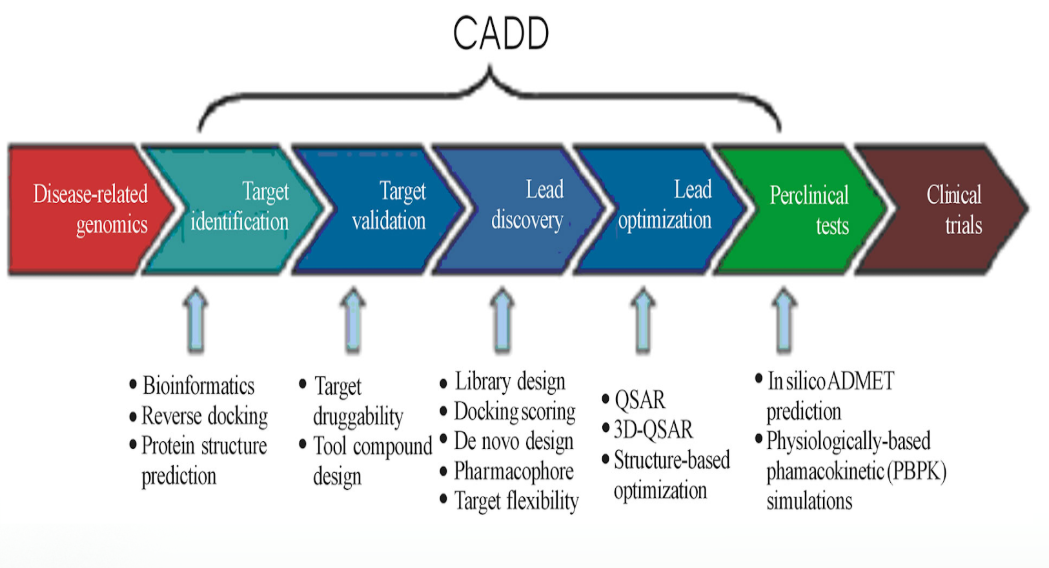
\includegraphics[width=15cm]{imagens/cadd.png}   
      \caption{Processo de desenvolvimento de fármacos}
    \cite{kore2012computer}
	\end{figure}
    
Nota-se o uso da técnica de docking molecular para a parte de identificação de alvos e na condução de descobertas, em ambos os casos é necessário estudar as propriedades químicas da estrutura que será analisada, seja na busca para otimização de uma proteína já conhecida ou não. 
O termo CADD (Computer-Aided Drug Design) refere-se ao processo de estudo de desenvolvimentos de drogas como um todo, podendo utilizar softwares para auxílio tendo maior precisão e rapidez nos resultados.

\section{Docking Molecular}
No final da década de 1980, surgiam os primeiros softwares que realizavam o processo de docking molecular, possibilitando desta forma trazer uma visão mais detalhada das estruturas. Com isso foi possível manipular as moléculas e otimizar as células com mais facilidade e simular com maior precisão, permitindo mais rapidez ao realizar testes virtuais.

Para realizar o docking, é necessário realizar o mapeamento das estruturas que irão se ligar, isso serve para prever os melhores pontos para que as moléculas se liguem, chamados de sítios de ligação, e conhecendo assim o ponto com melhor conformidade e qual a energia que será gasta para a união. Um exemplo de aplicação do docking pode ser visto na figura 1, onde mostra um ligante (inibidor) tentando se conectar a um receptor (prótese HIV), onde após a união é gerado uma estrutura única, chamada de complexo. Existem diversos pontos onde o ligante pode se conectar o que consequentemente gera inúmeros pontos de conformidade, com diferentes valores de afinidade.

      \begin{figure}[!htb]
      \centering
      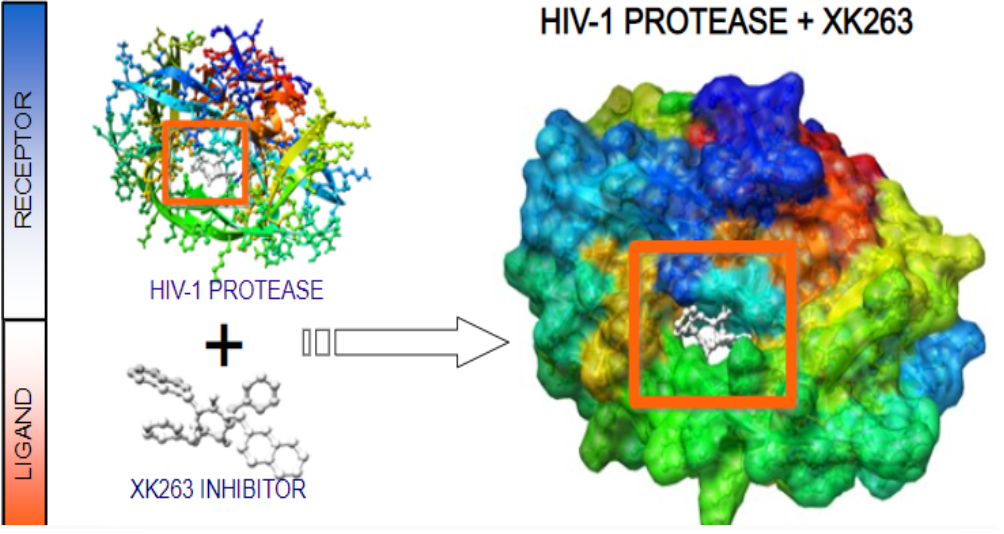
\includegraphics[width=13cm]{imagens/exemplo_docking.png}   
      \caption{Docking Molecular aplicado para estudo de inibidores de HIV}
    \cite{imagemDocking}
	\end{figure}
    \FloatBarrier
    
    
Tendo como objetivo analisar e prever a melhor conformidade entre duas estruturas celulares, conhecendo toda a região das moléculas dos ligantes e receptores, ao aplicar o docking é possível descobrir a afinidade de ligação que estas duas estruturas possuam entre si, podendo desta forma estimar o melhor encaixe.
Ao ocorrer uma ligação, é liberada uma certa quantidade de energia, esta energia é importante para medir a conformidade da união do complexo dessas duas estruturas (ligante e receptora).
Para realizar a medição, é utilizada funções de pontuação (score functions), focadas na minimização energética, que  segundo os trabalhos de\cite{lybrand1995ligand} e \cite{kitchen2004docking} , chegou-se a conclusão de que, quanto menor a energia gasta entre duas moléculas, melhor será sua a conformidade na união. 

Dependendo da estrutura que é analisada com o docking, torna-se possível criar uma substância capaz de inibir a molécula receptora, no caso de um inibidor de vírus por exemplo - \cite{ishikawa2011binding}

Com essa manipulação nas estruturas celulares, é possível destrinchar vários assuntos, pesquisas e artigos sobre os comportamentos de células e proteínas.
Esses exemplos são triviais para o estudo do comportamento das composições químicas das células para fazer medicamentos na área da biomedicina. 

Em geral a técnica de docking molecular é utilizada para desenvolver estruturas de células diversas; vírus de doenças, medicamentos, DNA e tudo que envolva fármacos. 

Muitos softwares já obtiveram resultados positivos ao utilizar docking, conforme mostrado na tabela 1, onde é listado exemplos destes softwares.
\begin{table}[h]
\centering
\begin{tabular}{@{}|c|c|c|@{}}
\toprule

Software & Alvo                   & Estudo                                                   \\ \midrule
Seed     & Plasmepsin             & Uma das causas da malária                                \\ \midrule
FlexX    & Fator de Edema Anthrax & Inibidor do edema                                        \\ \midrule
Glide    & Citocromo P450         & Deixa substâncias em formas hidrosolúveis         \\ \midrule
Surflex  & Topoisomerase I        & Otimização de anti-cancerígeno                           \\ \midrule
Dock     & Imunofilina F506       & Inibidor de calcineurina \\ \bottomrule
\end{tabular}
\caption{Softwares bem sucedidos ao utilizar docking molecular \cite{sliwoski2014computational} }
\end{table}

Para \cite{rodrigues2012estrategias}, o objetivo principal que se tem ao aplicar docking é aprimorar o processo de busca de novos candidatos a fármacos e acelerar o processo contínuo do seu planejamento. \\
Todos os fatores como as propriedades químicas das moléculas auxiliam a compreender de qual maneira se comportará as células, quais os tipos de ligação que podem ser utilizados como; proteína-ligando, proteína-DNA, proteína-proteína. \\Isso pode influenciar na abordagem de docking e afetar o desempenho nos softwares utilizados, ao serem aplicadas funções de pontuação.

Quanto a abordagem, existem duas formas bastante usuais para realizar o docking, uma delas pode ser classificada como Docking Rígido e outra como Docking Flexível.

No docking rígido os pontos de união de uma molécula ligante e receptora são mais limitados, isso se deve ao fato de existir uma menor liberdade em manipular as moléculas de uma célula, ou seja, a molécula ligante será rígida assim como o receptor. 
Consequentemente isso acaba resultando em maiores pontos a serem estimados, porque é necessário achar algum ponto do estrutura do ligante, onde exista uma boa superfície  e encaixe com a proteína, para então realizar a união de uma forma compatível. \\
Por procurar uma quantidade maior de locais (sítios de ligação), pode ser encontrado um lugar ideal e assim aumentar a precisão de acertos, já que existem vários pontos a serem avaliados e o que tiver menor energia deve realizar o acoplamento \cite{pagadala2017software}. 

Já no Docking Flexível, a molécula ligante pode ser manipulada e modelada com total liberdade para tentar se acoplar no receptor,  que neste caso continuará sendo rígido. 
O número de pontos a ser estimado será menor por não precisar procurar por superfícies compatíveis, pois pode ser ajustado o ligante ao receptor rígido.
Na literatura, é mais utilizado esta abordagem e em alguns casos pode ser feito novamente o processo de docking, porém dessa vez utilizando a abordagem de docking rígido, orientando o melhor resultado estimado anteriormente para que desta forma tenha-se uma boa conformidade.

Existe também uma abordagem que utiliza um pouco das ambas, docking rígido e flexível, chamada de docking induzido.
Para melhor entendimento dessas duas abordagens, é ilustrado abaixo  exemplos na figura 2, onde a estrutura receptora (em amarelo) e o ligante (vermelho) devem ter sempre buscar um bom encaixe para ter uma boa ligação. Nota-se que dependendo da abordagem, a estrutura de um terá que ser moldada para que tenha boa conformidade, a figura 2 ilustra o que ocorre ao escolher um sítio de ligação específico para encaixar um ligante a um receptor.


      \begin{figure}[!htb]
	\centering
	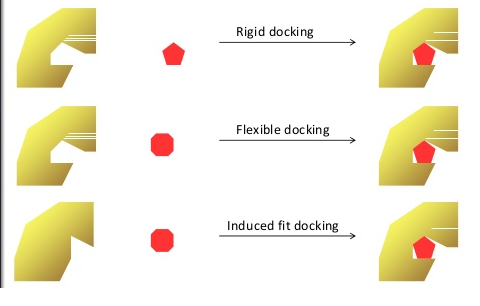
\includegraphics[width=15cm]{imagens/rigido_flexivel.png}
	\caption{Docking Rígido, Docking Flexível, Docking com encaixe induzido}
	\end{figure}
% figura retirada de (Não sei como citar, help! : https://www.slideshare.net/FlorentBarbault/molecular-docking-andvirtualscreening 

\section{Função de Pontuação}
O aprendizado de máquina se tornou algo bem comum ao ser aplicado em diversas áreas, para o caso de softwares que utilizem o docking, deve ser levantado os pontos que são relevantes para o processo de aplicação de docking.

Nos softwares de docking são utilizados algoritmos para gerar funções de avaliação para estimar o gasto energético durante a união entre moléculas, como por exemplo algoritmo genético \cite{holland1975adaptation}, Simulate Annealing \cite{kirkpatrick1984optimization},  algoritmo genético de Lamarca \cite{morris1998automated},  MonteCarlo \cite{caflisch1992monte}.

Estes algoritmos estão constantemente sendo evoluídos e até substituídos para obterem mais eficácia ao estimar grandes volumes de dados com um desempenho melhor.
Portanto, é possível dizer que ao melhorar a precisão desta função, é possível otimizar o processo de docking molecular consideravelmente.

\section{Software - Autodock Tools e Vina}

Um dos softwares mais populares utilizados para análise de resultados do docking, por pesquisadores e cientistas da área, é o Autodock Vina \cite{trott2010autodock}, que veio como parte do software dos mesmos criadores do Autodock Tools.

Neste software (Autodock)  é possível visualizar em 3D, sendo exibidas informações das coordenadas graficamente, permitindo assim reconhecer a posição de cada ponto da estrutura, e então manipular as moléculas de um determinado complexo, com o objetivo de poder estimar a energia gasta para realizar o acoplamento, podendo também,manipular a estrutura, adicionar ligantes , parâmetros extras,  emoção de átomos de água, escolher psítios de ligação para simulação.

Após essas modificações serem aplicadas, pode ser escrito, todas essas informações, em diversos arquivos de diferentes formatos, que podem ser lidos por outros softwares, como mostra a figura 3, neste caso está sendo salvo o arquivo em um formato lido pelo Vina, software responsável para estimação energética.\\Este mesmo é encarregado de calcular e estimar os melhores pontos de interação para ser realizado o docking, que baseado no arquivo salvo, contêm informações referentes ao posicionamento dos átomos do complexo, onde é calculada uma função de pontuação para prever em Kcal/s, a afinidade do complexo.

      \begin{figure}[H]
	\centering
	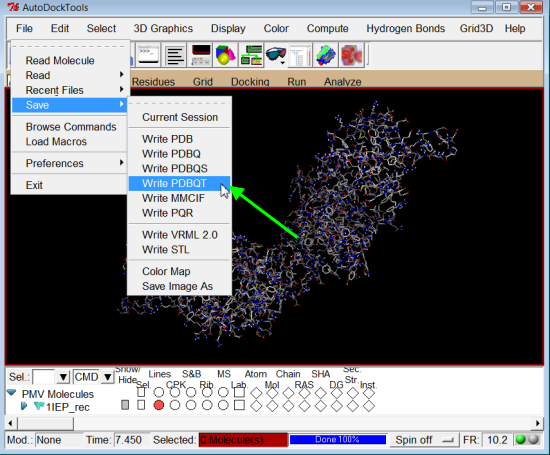
\includegraphics[width=0.90\linewidth]{imagens/Autodock.png}
	\caption{Salvando informações do complexo do tipo ligante-proteína no Autodock}
	\end{figure}
    \FloatBarrier

Este é o procedimento utilizado pelos cientistas e bio-tecnólogos ao utilizar estas ferramentas, logo após ser feita esta docagem simulada, é escolhido por especialistas os melhores resultados estimados pelo Vina, após diversos testes e assim feita a triagem em vitro, onde é tirada a prova real da qualidade das ligações.
Esta simulação do docking em softwares ajudam na busca por otimizações e composições de possíveis fármacos a serem estudados.

\section{Aprendizado de Máquina }

O foco foi direcionado para o estudo de uma das técnicas de aprendizado de máquina na literatura, em específico uma delas: o SVM, onde é possível utiliza-la para treinar os algoritmos para previsão e definição dos melhores resultados possíveis. 

Começando pelo básico, existe a divisão entre o aprendizado supervisionado, não supervisionado e por reforço.
Para este trabalho o foco foi estudar e explorar o aprendizado supervisionado, que utiliza funções de classificação e regressão\cite{boos2017funccoes},
com a finalidade de prever o melhor resultado estabelecido pela máquina.

Para estudar o comportamento de um complexo do tipo ligante-proteína em que será efetuado o docking, é necessário fazer um mapeamento de sua estrutura para compreender suas peculiaridades e comportamentos, tais como as propriedades químicas dos átomos. 
Tal processo é muito oneroso para processamento, levando muito tempo para que a máquina, reconheça padrões, aprenda como eles ocorrem e assim exibir resultados preditos, isso tudo pode variar, dependendo do poder de processamento e da técnica de machine learning utilizada (SVM, Algoritmo Genético,Random Forests).

Para fazer a máquina explorar e buscar informações referentes a composição das moléculas, é requerido bases de dados (data-sets), que contêm os dados necessários para efetuar treinos e testes \cite{chakrabarti2000data}.

Existem diversos softwares que utilizam técnicas de IA, cada um leva em consideração qual aspecto do docking deve ser melhorado. Abaixo é falado sobre alguns desses aspectos, segundo \cite{khamis2015machine}.

\textbf{(1)Poder de Pontuação:} Refere-se a habilidade de estimar diferentes poses de ligação para um determinado complexo de ligante-proteína. Com isso é possível fazer uma correlação para encontrar valores comuns e possivelmente prever diferentes resultados de afinidade.

\textbf{(2) Poder de Ranqueamento:}
É responsável por prever o valor mais próximo de energia gasta por cada complexo.

\textbf{(3)Poder de Docking:} Capacidade de identificar a melhor pose de conformidade para um dado ligante, através de um conjunto de poses geradas mostradas.

\textbf{(4)Poder de escaneamento:} Capacidade da função de pontuação descobrir e identificar os falsos positivos em uma determinada proteína alvo, junto a diversos conjuntos de moléculas distintas.

O foco deste trabalho foi estudar uma maneira para otimizar o poder de ranqueamento de docking, ou seja, ser capaz de avaliar e estimar qual o melhor resultado para uma estrutura de um determinada ligação ligante-proteína possa se encaixar, prevendo a afinidade ideal correspondente.

Para este caso em específico,\cite{ballester2010machine} utilizou florestas aleatórias e obteve um resultado satisfatório pois foi possível prever valores bem próximos de afinidade da maioria dos complexos, isso tudo ao utilizar uma grande quantidade de parâmetros e informações predispostas em uma base de dados bem conceituada chamada PDBBind, disponibilizada por \cite{wang2004pdbbind}.

\subsection{Random Forests}
Conforme visto na literatura, o desempenho das demais técnicas dependem da performance de execução dos diversos recursos computacionais empregados, ou seja, partindo do pressuposto da utilização da técnica de florestas aleatórias, também conhecido como random forests, não será necessário exímios recursos e processamento para melhores resultados, é evidente que quanto mais vezes for treinado, com mais amostras e melhor descrito estiverem os parâmetros, a eficácia será maior.

Dado o trabalho de \cite{ballester2010machine} como exemplo, foi necessário realizar validações nos data-sets e criar estruturas específicas com átomos específicos que estrutura ligante e estrutura receptora, para poder aplicar treinamentos nos data-sets.

As florestas aleatórias utilizam inúmeras árvores de decisão, onde cada uma produz uma resposta baseada nos parâmetros de entrada, e no final compreende-se que o valor mais comum entre todas as respostas seja o real -\cite{breiman2001random}
O uso de árvores de decisão pode trazer overfitting, devido a alguns fatores, como a forma que foi separada bases para teste e treino, poucos valores para teste e dificuldade em compreender parâmetros utilizados e por consequência acabar decorando os valores \cite{liaw2002classification}.

Isso pode ser reduzido com maior quantidade de valores distintos e aleatórios para amostras, tendo uma quantidade considerável de árvores, com valores aleatórios.

O trabalho de \cite{ballester2010machine} serviu como base de estudo, onde neste trabalho, será proposta uma alternativa a utilização das florestas aleatórias.

\subsection{Support Vector Machine}

A técnica de máquina de vetores de suporte, denominada svm, utiliza aprendizado supervisionado e é capaz de reconhecer padrões realizando classificação ou regressão e é uma das técnicas com melhores resultados apresentados \cite{lorena2007introduccao}. 
Esses padrões são reconhecidos através de exemplos que contenham parâmetros de entrada e um parâmetro de saída, este sendo chamado de label.

O svm separa os padrões que considera similares, e os coloca em uma classe específica, com isso ele cria modelos que ao serem treinados são capazes de predizer a qual classe um novo exemplo pertence\cite{boser1992training}.

Um clássico exemplo para demonstrar na prática o svm, é utilizando o data-set de Íris do \cite{fisher1936use} e aplicando diferentes kernels,  onde é separado em diferentes classes cada uma das espécies de flores (Iris-Virginica,Iris-Versicolor,Iris-Setosa), de acordo com o tamanho e comprimento como mostra a figura 5. 

    \begin{figure}[h]
	\centering
    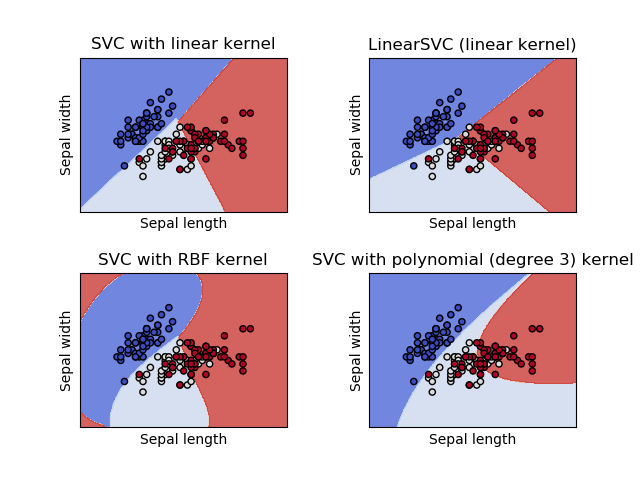
\includegraphics[width=0.90\linewidth]{imagens/exemplo_svm.png}
	\caption{Classificando por comprimento e largura com diferentes kernels}
	\end{figure}
    \FloatBarrier

Ao analisar a figura 5 é possível perceber que existe uma maior precisão de acertos de amostras ao utilizar diferentes tipos de Kernels.

Estes kernels possuem uma função específica, da qual são responsáveis por realizar a separação dos modelos do svm, e existem diferentes tipos; linear,gaussiano,polinomial e sigmóide, sendo o mais comumente empregado e testado em diversos outros estudos como o de \cite{huang2005extreme} e \cite{lima2014avaliaccao}.

Neste trabalho optou-se em utilizar o kernel Gaussiano do svm, descrito como RBF (radial basis function) , que demonstrou melhores resultados em comparação aos demais.

As informações presentes nas bases de testes e de treino foram armazenadas em uma tabela com parâmetros e labels, onde a afinidade do complexo constituem os labels e o restante, os parâmetros de entrada. 

Para todos esses parâmetros de entrada deve propor uma saída (Label),  com isso o svm irá realizar um treinamento utilizando uma análise de regressão utilizado o Kernel Gausiano como função principal.
Após ser realizado o treinamento é hora de predizer um valor para afinidade de acordo com os parâmetros informados.

\subsection{Validação Cruzada}

Para que melhorar a predição de modelos de treinamento e teste que utilizem aprendizado de máquina, é recorrente o uso de validações nos conjuntos de dados (data-sets), onde pode ser definidos vários grupos para treino e teste, com o objetivo de explorar ao máximo os parâmetros presentes no data-set.

Uma das validações utilizadas é a chamada validação cruzada \cite{kohavi1995study}, onde são separadas as amostras do data-set, em k grupos, sendo k a quantidade de grupos. Após a definição de quantos grupos existem, é treinado k-1 grupos e testado 1 grupo restante, em k iterações, mudando sempre o grupo para teste, este processo pode ser visto conforme a figura 6 onde k=5.

    \begin{figure}[h]
	\centering
    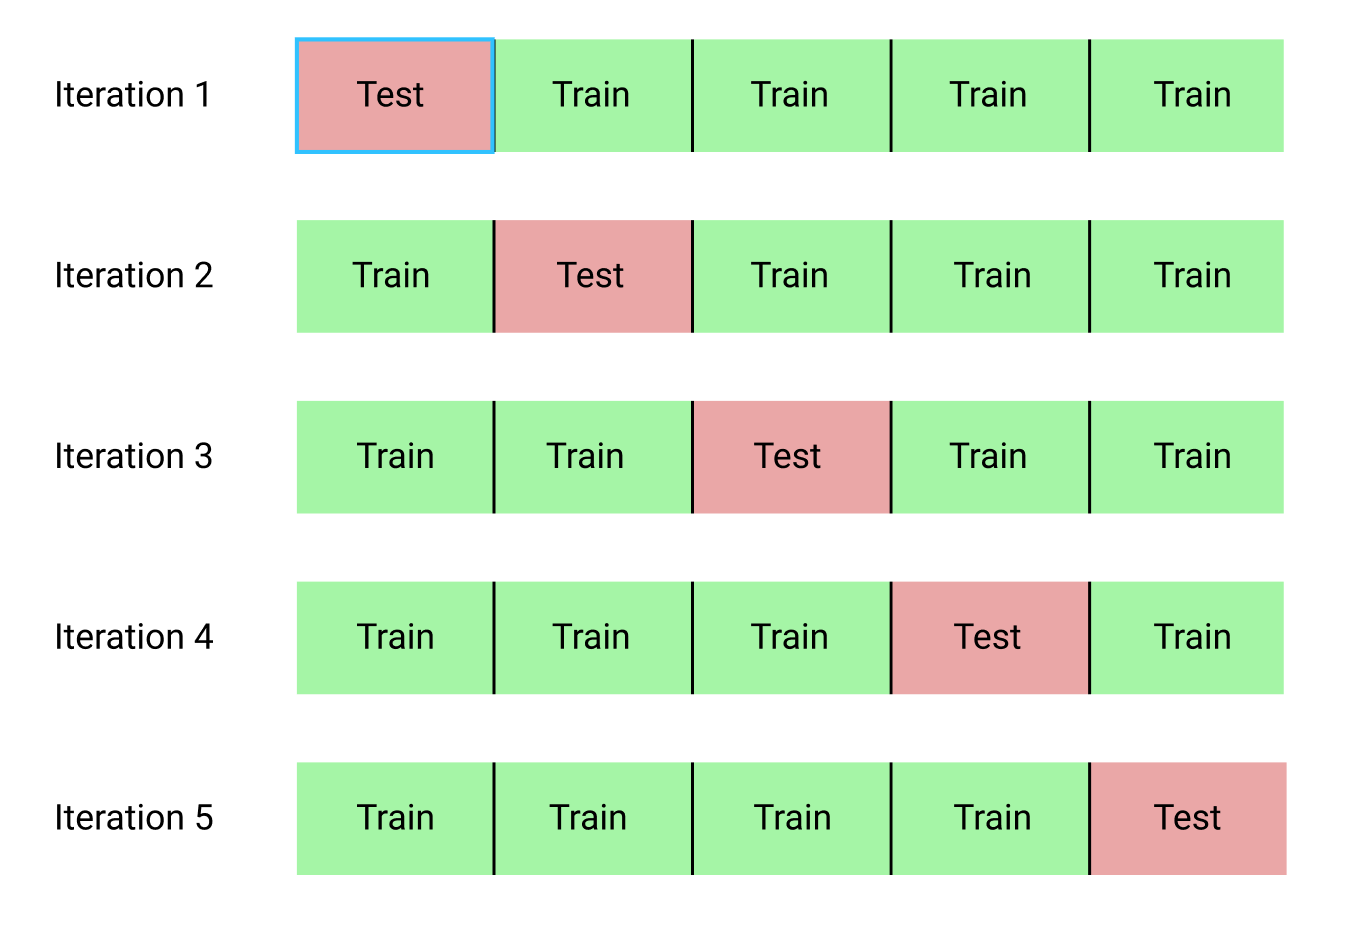
\includegraphics[width=0.90\linewidth]{imagens/cv.png}
	\caption{Etapas da validação cruzada}
	\end{figure}
    \FloatBarrier

Existem diversos métodos para executar a validação cruzada, sendo definidos como:

• K-Fold: separa em .

• Holdout: separa em .

• Leave-one-out: separa em .


\chapter{Metodologia}
Para este trabalho foi proposta uma alternativa ao RF-Score, algoritmo proposto por \cite{ballester2010machine}, que consiste em predizer um dado valor de afinidade para cada complexo do tipo ligante proteína.
Foi utilizado os mesmos dados dos data-sets para comparação e avaliação, buscando otimizar os resultados de treino e teste, ao aplicar uma outra técnica de machine learning, Suporte Vector Machine (svm), com a finalidade de resolver os problemas presentes na implementação de floresta aleatória.

Em primeiro momento o foco foi estudar os componentes necessários para realização de docking, realizando uma revisão bibliográfica dos recursos necessários para implementa-lo, como por exemplo, informações relevantes que podem influenciar resultados e previsões para treinamentos e testes. 

Esta revisão tem como objetivo se aprofundar nos temas que envolvem  o processo de docking, o contexto onde é aplicado, o processo que deve ser executado, as ferramentas, requisitos necessários  e saber quais os resultados esperados computacionalmente. 

O processo de realizar docking através de softwares, ajuda a compreender como ocorre o funcionamento desta técnica, com isso é possível ter uma estimativa de quais são os requisitos e resultados esperados que serão avaliados computacionalmente.

Após ser estudado o docking, foi feito uma revisão teórica com a finalidade de buscar e estudar, técnicas e trabalhos relacionados com o aprendizado de máquina.Tendo encontrado especificamente o conhecimento da técnica de florestas aleatórias em um trabalho relacionado de \cite{ballester2010machine} e tentando oferecer uma alternativa com a técnica do svm, onde ambos abordam temas como o a classificação das estruturas de proteínas bem como a predição dos melhores pontos estimados do docking.

Também foi feito um levantamento das ferramentas existentes; de quais ferramentas (softwares) são utilizados e quais foram as otimizações das funções de avaliação que tiveram ao longo dos anos segundo os benchmarks.

Assim como também testar e utilizar softwares,bases de dados, api's e frameworks de linguagens de programação, especificamente o módulo sklearn \cite{scikit-learn}, junto a linguagem de programação Python, que auxiliam no desenvolvimento e treino do aprendizado de máquina.
Onde todo o código feito está disponível no repositório Github - \citet{githubgianluca}.

\section{Criação de Data-sets}
É necessário ter uma grande quantidade de amostras prontas, onde cada uma possua um padrão que possa ser parametrizado, para poder aplicar o treinamento e teste, em um dado algoritmo que use alguma técnica de aprendizado de máquina.
Esses amostras são como exemplos de estudo para a máquina aprender, e estão presentes em um data-set, que seria um conjunto de dados, onde neste conjunto estão presentes diversas informações referentes a uma determinada amostra, quanto maior a quantidade de amostras presente em um data-set, melhor será o resultado do aprendizado. 
% colocar imagem ? Opcional

Os data-sets utilizados neste trabalho podem ser obtidos em \citeauthor{sitepdbbind}, onde possui diversas versões de bases de informações, onde foi utilizado a versão refinada de 2007. \\
Essas bases contêm todas as informações, como posição, tipos e propriedades químicas do átomo de cada molécula que compõem uma determinada estrutura.\\
O uso dessas bases é de extrema importância, pois ao utiliza-la será possível aplicar treinamento e com isso estimar resultados no ao realizar um teste. 

Para este trabalho, os data-sets foram organizados da mesma forma que o trabalho relacionado de \citeauthor{ballester2010machine}, conforme explicado abaixo e mostrado na figura 6, com o objetivo de aplicar treinamento e teste com a técnica de svm e realizar uma comparação com a técnica de florestas aleatórias do trabalho relacionado, onde serão vistos os resultados no Capítulo 4.

Essas bases contém complexos de proteínas-ligantes, e foram validadas com uma série de critérios descritos por \cite{cheng2009comparative}, pois as informações são muito heterogêneas, até mesmo para um processamento de técnicas de machine learning. 
Segue abaixo estes critérios adotados para criação desta base:

\begin{enumerate}
\item Apenas o complexos proteína-ligante cujas estruturas são determinadas através de difração de cristal foram considerados. Cada estrutura qualificada como complexa, deve ter uma resolução global melhor do que ou igual a 2,5 Å.
 Além disso, tanto a proteína como o ligando precisa estar completo na estrutura cristalina.
\item Preocupações sobre a qualidade dos dados de ligação. Apenas o complexos proteína-ligante com constantes de dissociação conhecidas (Kd) ou constantes de inibição (Ki) foram consideradas. Além do que, tanto a proteína como o ligante utilizado no ensaio de ligação tem que corresponder exatamente aos usados na determinação da estrutura.
\item Preocupações sobre os componentes dos complexos. Somente os complexos de proteína-ligante ligados de forma não covalente foram considerados. Cada complexo qualificado deve ser formado por um molécula de proteína e uma molécula de ligando de uma maneira binária. Em outras palavras, não deve haver vários ligantes ligados nas proximidades de um local de ligação comum. O ligando molécula não deve conter elementos incomuns, como como Be, B, Si e átomos de metal.
\end{enumerate}

Para aplicação deste estudo foram utilizadas estas duas data-sets, uma chamada de refinada, que será utilizada para treinamento e outra chamada core que será utilizada para teste. \\Isso é ilustrado na figura 5, onde a base refinada originalmente continha cerca de 1300 linhas de exemplos com os parâmetros descritos anteriormente, porém foram retirados e separados em 3 clusters com 65 complexos da mesma, que acabou sendo utilizada para o teste, que será chamada de core. \\Logo existem  2 data-sets, um para treino com 1105 amostras (refinado) e outro para teste com 195 amostras para teste. 

    \begin{figure}[h]
	\centering
    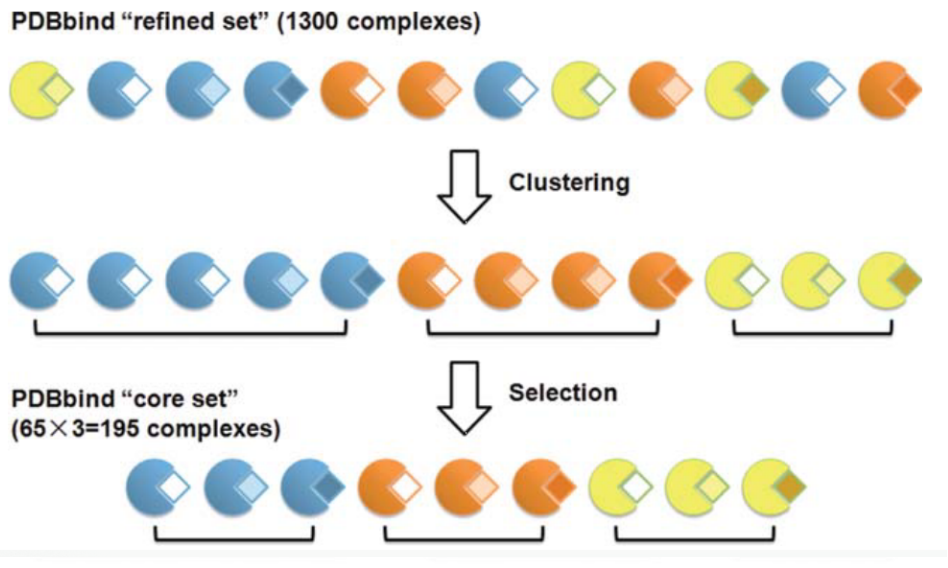
\includegraphics[width=0.90\linewidth]{imagens/data-set.png}
	\caption{Separação de data-sets de treino e teste}
	\end{figure}

\section{Definição de Parâmetros}
Seguindo o exemplo de \cite{ballester2010machine}, foram coletados a afinidade, de cada complexo dos arquivos presentes na base do PDBbind (cada linha possui um complexo).

Também foi calculado a distância euclidiana entre as interações dos átomos de C,N,O,F,P,S,Cl,Br,I (somente daqueles) que compõem a estrutura do ligante e da proteína.

Um parâmetro na data-set será responsável por identificar a qual proteína é correspondente, ou seja, o Id do complexo (11gs por exemplo).

Para a afinidade é utilizado as constantes Kd(constante de dissociação), Ki (constante de inibição) e IC. 
Dependendo da estrutura só será informada alguma destas constantes, com é atribuído como valor de afinidade o resultado do -log10 K, sendo K a constante que estiver presente.

Para a distância eucliana de cada átomo será utilizado 36 campos de parâmetros que representam a distância entre um e outro, por exemplo a distância entre o átomo C e N representa um valor, C e O também e assim sucessivamente, resultando em 36 valores. 

\section{Pseudocódigo}

Colocar assim ou tirar print da IDE
início\\
 variavel dataframe dataset\\
 variavel vetor X\\
 variavel vetor Y\\
 ler dataset\\
 dividir data-set em pedeços\\
 X = parametros data-set\\
 Y = labels data-set\\
 cria modelo de svm  \\
 ajusta svm com X e Y\\
 prediz Y com X\\
 calcular RMSE\\
 plotar gráfico\\
fim\\

\section{Bibliotecas e API's para SVM}

Nesta parte é mostrado as ferramentas necessárias para construir o algoritmo de machine learning e avaliar resultados.

\subsection{Python}

A linguagem Python, versão 3, é de alto nível, com ênfase em manter o código legível e fácil de entender,  expressando programas em poucas linhas de código quando é comparada a programas feitos em outras linguagens.

Foi criada por Guido van Rossum, na década de 80 e hoje, sua licença é administrada pela Python Software Foundation,\cite{pythonfundation} que permite seu uso até para fins comerciais, e seu desenvolvimento é mantido por uma comunidade, uma vez que a linguagem é open-source.

Python é uma linguagem de tipagem dinâmica, projetada para atender a diferentes paradigmas de programação como o imperativo, o orientado a objetos e o funcional. 
Seu interpretador pode ser instalado em diferentes sistemas operacionais para a execução dos programas escritos.

É uma linguagem rica em bibliotecas próprias e também conta com diversas api's, módulos e frameworks desenvolvidos por terceiros, estendendo sua aplicação a diversas áreas, como desenvolvimento Web, análises científicas , cálculos numéricos, desenvolvimento de jogos entre outros.

Entre suas inúmeras bibliotecas e ferramentas, existem várias que são voltadas para a mineração de dados, a aprendizagem de máquina e o processamento da linguagem natural.

O Python hoje em dia é bem popular hoje em dia, por conta disso existe inúmeros tutorias e vídeos explicativos que são facilmente encontrados pela internet.

\subsection{Pandas}
É uma biblioteca escrita em linguagem Python, para análise de dados em alta performance. Utiliza o pacote padrão do Python, NumPy, para computar cálculos científicos.

A biblioteca Pandas fornece estrutura de dados novas e ferramentas para sua manipulação, provendo maior facilidade na execução das análises desejadas podendo ser integrada outros módulos com gráficos similares aos do Matlab.

Neste trabalho foi utilizado uma tabela da biblioteca, chamada de data-frame. O data-frame é possui uma estrutura com indexação integrada, sendo basicamente, uma estrutura com linhas e colunas onde cada coluna tem um índice, associado a um conjunto de valores. 

Cada linha, portanto, tem vários valores, um deles referente a cada coluna indexada do data-frame.

A biblioteca Pandas é importante para a leitura e organização dos dados brutos das bases de dados, indexando cada uma delas pelo seu rótulo, separando parâmetros e labels, transformando o conjunto inicial em algo mais fácil de ser manipulado por outras funções.

\subsection{Scikit-Learn}
Possui um conjunto de ferramentas para mineração e análise de dados, constituindo uma mistura de vários pacotes como NumPy, SciPy e matplotlib. \\
Os principais recursos do Scikit-Learn são algoritmos para:

• Clusterização: processo de agrupamento de objetos com características similares.

• Regressão: para predição de atributos de valores contínuos para objetos a eles associados.

• Seleção de modelos: módulos para comparação e validação de parâmetros e modelos,tais como a validação cruzada.

• Redução de dimensionamento: ou diminuição do número de variáveis a serem consideradas para estudo.

• Pré-processamento: preparação dos dados, extração do vetor de características e  normalização.

• Classificação: métodos de atribuição de um dado a um conjunto específico, tais como o svm, que aqui será o foco na elaboração do estudo.

Neste trabalho será utilizado a Regressão para a predição de valores de afinidades dos complexos.

\chapter{Resultados}
Neste capítulo serão apresentados os resultados deste trabalho ao aplicar a técnica de svm, comparando com o trabalho relacionado de \citeauthor{ballester2010machine}, onde o mesmo utilizou a técnica de florestas aleatórias. 
Em ambos os trabalhos foram adotadas bases do PDBBIND no ano de 2007, e utilizam os mesmos parâmetros para aplicar treinamento e teste de aprendizado de máquina.
O objetivo de ambas as técnicas, é medir o índice de acertos entre afinidade real e a afinidade prevista pelo algoritmo.
Como métrica de desempenho será utilizado o RMSE (root-mean-square-error), ou seja, o erro médio quadrático.

\section{Resultados das Florestas Aleatórias}

No trabalho proposto por \textbf{\cite{ballester2010machine}}, foi executado um treinamento utilizando 1105 amostras obtendo um RMSE=0.74 e um teste utilizando 195 amostras com um RMSE=1.58, isso pode ser ilustrado pela figura 7, onde é traçada uma reta com os valores reais (y) e valores preditos (x) pelo algoritmo de florestas aleatórias, quanto mais próximo os pontos estão da reta mais corretos os valores preditos estão.
    \begin{figure}[h]
	\centering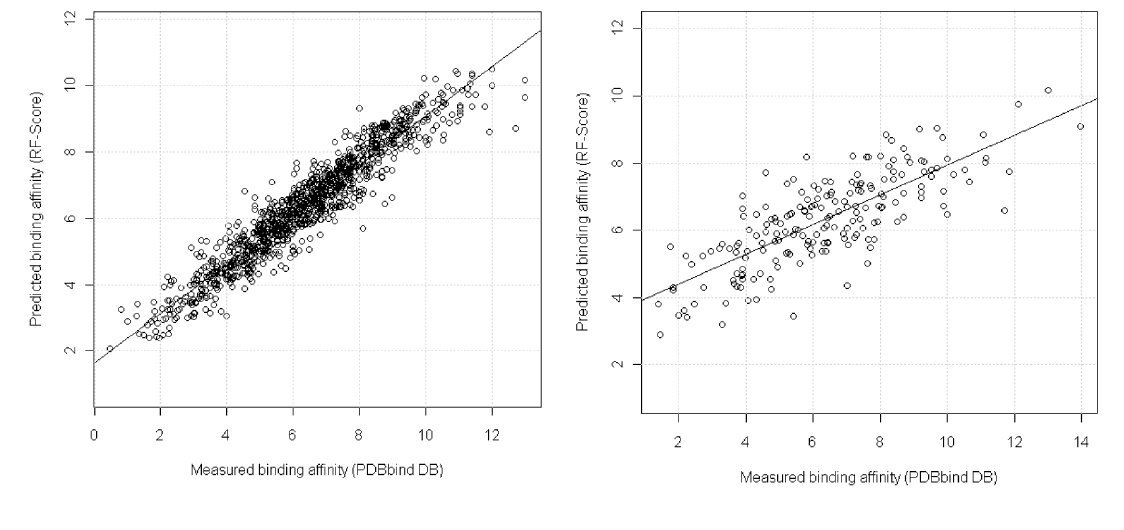
\includegraphics[width=17cm]{imagens/treino_teste_ballester.png}
	\caption{Treino E Teste com Random Forests}
	\end{figure}
    \FloatBarrier

\section{Resultados do SVM}

Da mesma forma que foi descrito os resultadas das florestas aleatórias, está separado o mesmo número de amostras para treino e teste ao aplicar o svm, obtendo um RMSE=0.45 e RMSE=1.97 respectivamente, onde pode ser vistos a reta na figura 8.
	\begin{figure}[!h]
	\centering
	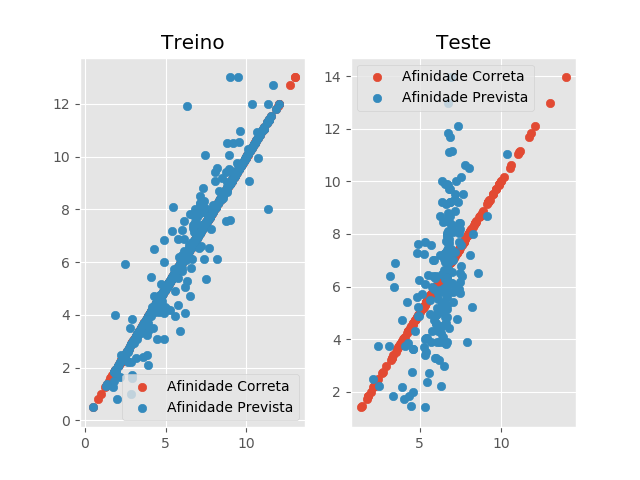
\includegraphics[width=15cm]{imagens/teste_treino_meu.png}
	\caption{Treino e Teste com svm sem validação cruzada}
	\end{figure}
    \FloatBarrier
    
Ao analisar a figura 8, nota-se que não houve uma esperada melhora no teste ao aplicar o svm se comparada com a figura 7, em decorrência disto foi aplicada uma validação cruzada, utilizando o método k-fold, sendo separados as 1300 amostras em 130 grupos, contendo 10 amostras cada.

    \begin{figure}[!h]
	\centering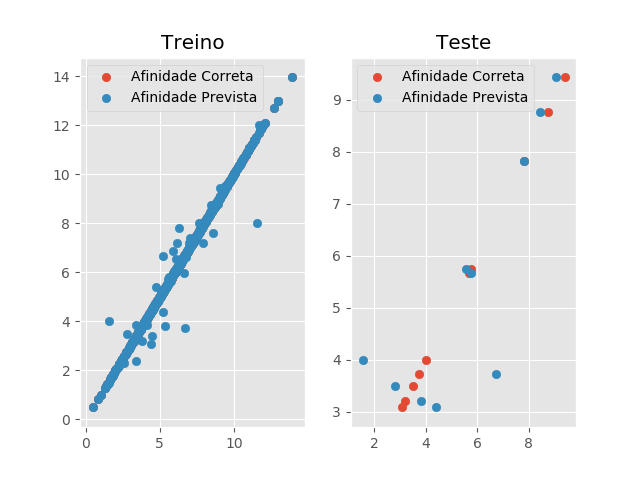
\includegraphics[width=15cm]{imagens/svmCV.png}
	\caption{Treino e Teste com svm e validação cruzada}
	\end{figure}
    \FloatBarrier
    
Por conta da aplicação desta técnica, o número de amostras para teste ficou menor como mostra a figura 9.    

\section{SVM X Random Forest}
Inicialmente ao utilizar o data-set sem a validação cruzada, nota-se que a técnica de Random Forest possui menor RMSE no teste, isso caracteriza menor índice de erros e consequentemente melhores resultados preditos.
Diferentemente no svm, percebe-se que a previsão para de treinamento foi superior, RMSE=0.45 (svm) contra 0.74(florestas aleatórias) embora isso não seja tão relevante para uma possível aplicação, já que no teste ocorre uma maior falha ao prever resultados, com 1.97 do svm contra 1.58 das florestas aleatórias, conforme mostra a tabela 2.

\begin{table}[h]
\centering
\begin{tabular}{@{}|c|c|c|@{}}
\toprule
Autor 		 					  & Ballester                           &  Gianluca                                                \\ \midrule
Técnica     					&  Florestas Aleatórias       &  Support Vector Machine                      \\ \midrule
RMSE Treinamento    & 0.74 									 & 0.45                                        					   \\ \midrule
RMSE Teste    				&  1.58         						 & 1.97         													\\ \midrule
\end{tabular}
\caption{Comparação de Resultados deste trabalho com o de Ballester}
\end{table}

Porém, ao aplicar uma técnica de validação cruzada para a base de dados refinada é possível notar que os resultados melhoram consideravelmente, conforme mostra a tabela 3.

\begin{table}[h]
\centering
\begin{tabular}{@{}|c|c|c|@{}}
\toprule
Autor 		 					  & Ballester                           &  Gianluca                                                \\ \midrule
Técnica     					&  Florestas Aleatórias       &  Support Vector Machine                      \\ \midrule
RMSE Treinamento    & 0.74 									 &  0.14                                       					   \\ \midrule
RMSE Teste    				&  1.58         						 & 1.33         													\\ \midrule
\end{tabular}
\caption{Aplicando Validação Cruzada no data-set refinado}
\end{table}

Em resumo, o trabalho proposto por \citeauthor{ballester2010machine}, possui melhor RMSE para predição de valores de afinidade dos complexos do tipo proteína-ligante, sem aplicar uma validação de data-sets. \\
Consequentemente, isso pode trazer valores de informações repetidos do treino para o teste, fazendo com que o algoritmo apenas decore a informação (overfitting), não identifique padrões e faça a predição de valores incorretos.\\
Utilizando a técnica de validação cruzada nos data-sets, o valor do RMSE diminuiu comparado ao teste de \citeauthor{ballester2010machine}, tendo 1.33 contra 1.58.


\chapter{Conclusão}
Neste trabalho foi realizado um estudo de diversas áreas; biomedicina, inteligência artificial, programação e estatística. Todas com a finalidade de otimizar a predição de afinidade dos complexos do tipo ligante-proteína.

Foi explorado e testado diversos kernels e parâmetros do svm, do qual serviu para aumentar o nível de conhecimento elucidado para elaboração deste trabalho. 

Para superar o algoritmo de florestas aleatórias de \citeauthor{ballester2010machine}, foi necessário aplicar uma validação nos data-sets, utilizando a técnica de validação cruzada, diminuindo o valor de RMSE=1.58, com o algoritmo de svm realizado neste trabalho que obteve RMSE=1.33.

Conforme foi visto ao longo deste trabalho, sempre irão existir avanços que possibilitem o uso de novas tecnologias, neste trabalho em especial, no docking molecular.

A tendência é que futuramente exista avanços nas áreas de aprendizado de máquina e biotecnologia, permitindo trazer maior volume de informações e técnicas que otimizem ainda mais o processo de avaliação do docking molecular e assim melhore o processo de desenvolvimento de fármacos.

\section{Trabalhos Futuros}

Apesar de ter todo esforço e evolução da área de inteligência artificial, muito falta para ser alcançado, a extração de informações ainda é pequena e bastante heterogênea para um processamento avançado, o que traz por consequência uma falha muito grande em prever resultados reais para aplicações da biomedicina no dia-a-dia.
Para um novo trabalho, deverá ser explorado outra técnica de aprendizado de máquina que apresente melhores resultados, como o uso de Redes Neurais profundas, contando com mais informações presentes em bases de dados mais recentes, para que dessa forma ocorra uma melhora significativa no treinamento e teste, prevendo melhores resultados.

\bibliography{relatorio}
\bibliographystyle{abnt}
\end{document}

